\chapter{Implementation}
\label{chapter:implementation}

% This chapter should include design choices for my implementation. For
% example choices taken for generating relevant data for test users
% and a computational sound method for doing so. As JavaScript in browsers are
% quite inefficient it will probably be necessary to persist data at a server
% in some sort of cache. The clients could then get this data by invoking a
% single request. The result could for instance be JSON serialized. Scraping
% of such data is probably done more efficient and safer at the server side
% since multiple XMLHttpRequest in the clients for scraping and parsing could
% prove to be quite computational expensive.

As we've seen in 
\sectionref{building.on.top.of.the.web}
it's possible to build applications on top of existing web sites by creating
transparent prototype implementations. This chapter starts with an account of
what kind of navigation system we wanted to build, goes on to describe why we
decided on such navigational designs, and concludes with an explanation of how
the implementation was built\dash{}the ingredients of our implementation.

\section{Design}

% no new data. making existing data more readily available.
%
% try to say something about how less data makes choices easier
% to make -- something a interaction feed will try to solve
%
% try to cite and include anecdotes from
% the paradox of choice: why more is less
%
% You know you?ve achieved perfection in design, not when you have nothing
% more to add, but when you have nothing more to take away.
%   -- Antoine de Saint Exupery (The Little Prince)

\section{Process}
% Prototype, exploratory
% TDD, BDD

\subsection{Prototyping}

A \term{prototype} is an early version of an application that are used for
finding out more about the problem at hand and it's possible solutions
\citep[p.~409]{sommerville07}.
The software developed for our research on social navigation fits these
characteristics. It's not supposed to be used after it's behavior is
evaluated. For that it's to inefficient and relies on specific web browser
environments and extensions. This does not mean that the prototype can't have
impact on how \urort{} evolves in the future. If our evaluation favors our
design decisions the developers of \urort{} might take advantage of such
potential improvements in their web site design.

\citet[pp.~409--410]{sommerville07} explains that a prototype can be used for
\begin{inparaenum}[(i)]
  \item gathering more sound requirements from users during a
    requirements phase,
  \item evaluating the feasibility of a proposed design during a
    design phase, and
  \item testing the final system by verifying it against the prototype.
\end{inparaenum}
We're following his second example of prototype usage by making a prototype
for what we believe to be a sound social navigation design. This is then
evaluated. If time permitted (sadly one has limited time and resources
available during master thesis research) the results of such an evaluation
could be input in a new design process and a new prototype system.

As \citet[p.~114]{mcconnell04} explains prototyping can mean different things
based on context. Often it's used to explain systems where one writes the
least amount of code to get a solution and throw it all away when the design
question is answered. This is not our intention. We'll try to make the system
fully operational and make the code we author comprehensible and
valid. More precisely we're creating a \term{high-fidelity} prototype
\cite[p.~78]{rudd96} with a robust architecture.

\subsection{Testing}


\section{Architecture}

Our implementation basically needs to do two things:

\begin{enum}
  \item Collect existing data from various places on the \urort{} web site.
  \item Display this data in existing web pages on the \urort{} web site in
    a way that we hope will enhance navigation.
\end{enum}

\subsection{Client-Server Model}

A client-server model is an architecture where one is separating a system into
two logical parts: a client and a server \citep[p.~3]{lewandowski98}. The
client is a \openpostquote[p.~11]{malkin96}{%
  computer system or process that requests a service of another
  computer system or process}
and the server is a \postquote[p.~49]{malkin96}{%
  provider of resources}
They have disparate responsibilities, the client is a consumer and the
server is a producer \citep[p.~3]{lewandowski98}. This delegation is the
essential part of client-server computing and enables one to focus on one
aspect of a problem as one does when adhering to the concept of
\term{separation of concerns} \citep[p.~61]{dijkstra82}.
A client-server model also enables one to scale both horizontally and
vertically%
\sidenote{
  To scale horizontally entails adding more servers to a client-server
  architecture. When one increases the resources of a single server
  one is scaling vertically.
},
an impossible feat with monolithic systems \citep[pp.~7--8]{lewandowski98}.

We therefore decided to use a client-server architecture so that we could
offload some of the more computationally expensive operations off the client
and onto a dedicated server. Another benefit of such an architecture is that
it allows us to cache data globally\dash{}shared by all clients. This means
that data collection is handled on the server side, while data display
obviously is handled on the client side.

\citet[p.~887--888]{nishimoto06} implemented a system for refinding places one
have already visited on the Web. What's interesting about their system is that
their architecture is strikingly similar to our own. They use a
client-server model with a user-script enabled browser as their client. The
client facilitates the users as they're navigating by supplying additional
information alongside existing web pages. One of the ingredients in helping
users in their browsing is suppling information from third party content
providers. By seperating this computationally heavy part of the application
into the server side they were able to offload the clients in a similar
manner we inteded when fetching data from \urort{}.

With all the pieces in place of our third party software puzzle described in
\chapterref{selection.of.third.party.software}
we present a high level view of the architecture, from the client to the
server, in
\figureref{fig.prototype.architecture}.

\begin{figure}
  \begin{whole}
    \centering
    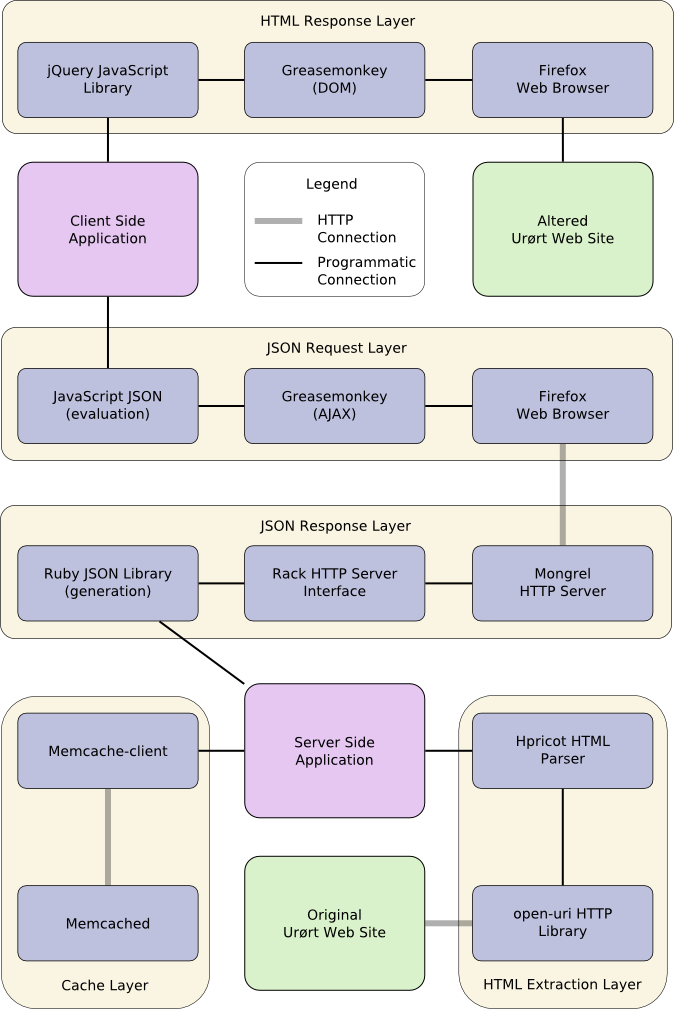
\includegraphics[width=0.9\wholewidth]{fig_prototype_architecture}
    \caption[Prototype Architecture]{
      High level view of the overall prototype architecture.
    }
    \label{figure:fig.prototype.architecture}
  \end{whole}
\end{figure}

\subsection{Caching}
% write about the cache and what is done on a \term{cache miss}. Also give
% reasons for \term{time to live}.

\subsection{Asynchronous Requests}

In the traditional style of \abbr{AJAX} applications we request information on
the client side of our prototype asynchronous%
\sidenote{
  While it's possible to use synchronous requests with \code{XMLHttpRequest}
  it's strongly discouraged since the entire web browser will be locked
  while it's waiting for a response for it's request \citep{crockford06a}.
}.
This means that requests handled by the \code{XMLHttpRequest} object
are independent of other requests the browser is making\dash{}they
are non-blocking. This enables developers to create web pages where additional
data is requested after the page is loaded by a normal \abbr{HTTP} request.
This is often coupled with the ability to detect user behaviour, and contents
are requested only when needed. \citet[pp.281--282]{stamey06} argues that
the increased complexity (and thereby size) of todays web pages have created
problems in percieved responsivness for users due to network latency. He
tinks asyncronous request of small content items solves this
problem\dash{}bringing greater interactivity to the user. Another solution
that can be combined is to move some processing into the client with
JavaScript \citep[p.~9]{jazayeri07}

\subsection{Modularization}

% ruby modules, classes, separate files and directories
% packaged up with rubygems to make exchange and installation of the software
% easier.
% javascript packaging necessary? only downloaded once. gzip compression not
% an option. maybe minifying or deep packaging processes?
% maybe MVC: reenskaug79

\subsection{Data Structure}
% the structure of our persistent data
